\chapter{Solution Design}

This chapter aims to fully describe the solution design from a top to bottom approach. First of all, the general idea of the design is described, abstracting every detail to easily understand the whole. Later on, the different sections of the design are explained with all their characteristics described. The implementation details are left for the following chapters, whereas here we only focus on the ideas and methods used.

In short, the solution to the problem of studying what an observer near a black hole would see is a ray tracer, that is, a device that computes the origin of the rays of light that arrives to a virtual camera placed in a virtual universe.

This work implements a general relativity ray tracer; \ie, a ray tracer for which the path followed by light is not always a straight line.

In \autoref{sec:gendesc}, the layout of the solution is depicted, whereas in \autoref{sec:parallel}, the parallelization designed is explained. \autoref{sec:pinhole} explains the pinhole camera model, describing the identification of each pixel on the camera with a lightlike particle coming from the celestial sphere. Finally, \autoref{sec:initcond} and \autoref{sec:numerical} describes the necessary work to numerically solve the geodesic equations.

\section{General Description}
\label{sec:gendesc}

Imagine a spacetime defined by a Kerr metric, with a black hole on its centre, and a camera with a digital sensor placed near it.

As we have studied, all rays that hit the sensor have followed a geodesic to finally arrive to the camera, and their paths are of great interest for us: the origin of the ray will tell us what the particular pixels see and the curvature of the geodesic will let us understand the geometric nature of the spacetime.

For every pixel on the sensor, the ray tracer work can be abstracted as a function that computes the path of the ray that hit it. Therefore, from the pixel coordinates, $p = (p_x, p_y)$, it computes the geodesic path followed by the ray.

This point is computed using the \ac{ODE} system described in \autoref{theo:eqsmotion}, derived from the Kerr spacetime. Therefore, a numerical solver for such systems is needed, along with the initial conditions of each ray. This conforms an \ac{IVP}, a kind of well-known problems whose numerical solutions are widely studied.

Abstracting all these tasks out, the general outline of the ray tracer is described on \autoref{alg:raytracer}.

\begin{algorithm}
	\caption{High-level abstraction of the ray tracer}
	\label{alg:raytracer}
	\begin{algorithmic}[1]
		\Function{Ray Tracer}{}
		\State ODEsystem $\gets$ Geodesics equations for the Kerr spacetime
		\State Camera $\gets$ Pinhole camera model
		\State Geodesics $\gets \{\emptyset\}$
		\For{pixel $p = (p_x, p_y)$ in the Camera sensor}
			\State initCond $\gets$ initConditions($p_x$, $p_y$)
			\State $\gamma_{xy} \gets$ solveInitValueProblem(ODEsystem, initCond)
			\State Geodesics $\gets$ Geodesics $\cup$ $\gamma_{xy}$
		\EndFor
		\Return{Geodesics}
	\EndFunction
	\end{algorithmic}
\end{algorithm}

The solution designed for the ray tracer is based on the algorithm described in \cite{thorne15}, that assumes the following:
\begin{enumerate}
	\item The spacetime is defined by the Kerr metric written in \ac{BL} coordinates (see \autoref{eq:kerrmetric}), with a black hole in the centre of the spatial coordinates parametrized by its spin $a$. Its mass is assumed to be 1.
	\item The \ac{FIDO} is a locally non-rotating observer. We define a family of \ac{FIDO} at rest in space with orthonormal basis vectors $\{e_r, e_\vartheta, e_\varphi\}$, pointing along the spatial coordinate lines.
	\item A camera is placed outside of the horizon of the black hole.
	\begin{enumerate}
		\item The position of the camera is described by the coordinates $\{r_c, \vartheta_c, \varphi_c\}$.
		\item The camera speed with respect to the \ac{FIDO} is noted as $\beta$.
		\item The direction of motion relative to the \ac{FIDO} is described by a unit vector $B$ in the camera's reference frame.
		\item We set up a right-handed coordinate system placed on the camera's reference frame, with the orthonormal basis $\{e_x, e_y, e_z\}$, where
		\begin{itemize}
			\item $e_y$ is identified with $B$; \ie, it points to the direction of motion of the camera.
			\item $e_x$ is perpendicular to $e_y$ and contained on the plane $\langle e_{\widehat{r}}, e_{\widehat{\vartheta}} \rangle$.
			\item $e_z$ is perpendicular to $e_x$ and to $e_y$.
		\end{itemize}
		\item We set up a spherical coordinate system derived from the previous one, noted as $\{\vartheta_{cs}, \varphi_{cs}\}$, where:
		\begin{itemize}
			\item $\vartheta$ is the polar angle with respect to the coordinate system origin.
			\item $\varphi$ is the azimuthal angle with respect to the coordinate system origin. The black hole is assumed to rotate in the positive $\varphi$ direction.
		\end{itemize}
	\end{enumerate}
\end{enumerate}

The algorithm consider a set of timelike geodesics arriving at the camera. These geodesics are then integrated backwards to obtain the ray's point of origin on the celestial sphere (at $r = \infty$). These points are noted as $(\vartheta', \varphi')$.

In short, the algorithm goal is to compute the following map
\begin{equation}
	\label{eq:initmap}
	(\vartheta_{cs}, \varphi_{cs}) \xmapsto{\mathfrak{h}_1} (\vartheta', \varphi')
\end{equation}
for each considered geodesic arriving at the camera.

\section{Parallelization Techniques}
\label{sec:parallel}

A ray tracer is in general highly parallelizable, and our design is not different: it performs the exact same operation on a large set of different data, namely it solves the \ac{ODE} system, whose equations (\autoref{theo:eqsmotion}) are always the same, on a large number of different initial conditions.

The idea behind the parallelization design is easy: for each parallelized node, we have to feed the numerical solver with a different initial condition, computed from each pixel of the image. Using the classic Flynn's taxonomy \cite{flynn72} terminology, our architecture follows a \ac{SIMD} paradigm, where a single generalized task works on multiple data streams in order to compute multiple results.

Ideally, we would like to design a completely parallel solution, in which we have the same number of nodes in the parallel architecture as pixels we have in the image. Although this is highly difficult for large images with the classic parallelization on \acp{CPU}, the new \ac{GPU} techniques will help us get closer this goal.

\subsection{General-Purpose Computing on Graphics Processing Units}

Historically, \acp{GPU} have been used to process tasks and data always related to computer graphic purposes, whereas \acp{CPU} have been used in general computation.

In recent years, a new powerful technique has been deeply studied: the so-called \ac{GPGPU}. Its goal is to use the \acp{GPU}, designed to have thousands of cores that can process data in parallel, to general purpose computing, not only computer graphics tasks.

Although each of the cores on a \ac{GPU} is much less powerful than a single \ac{CPU}, the great order of parallelization ---thousands of cores in a \ac{GPU} against just a few dozens of them on \acp{CPU}--- and the specific design to handle a parallel architecture makes the use of \ac{GPGPU} appealing when one want to design an efficient solution.

Our ray tracer uses this paradigm, virtually parallelizing the computation of each geodesic in a different \ac{GPU} core. We say \emph{virtually} because the number of cores in a \ac{GPU} is always finite, and for large images, some computations will have to be serialized. However, as we will see in the following chapter, this will be transparent to us, developers, by using a proper \ac{GPGPU} library.

\subsection{Parallelized Solution}

With this paradigm in mind, we can describe the parallelized solution by modifying the main loop on \autoref{alg:raytracer}, whose iterations will be split across all the nodes on the \ac{GPU}.

If we abstract the computation of the geodesic that hits one single pixel in a function, as shown in \autoref{alg:onepixel}, we can finally define the layout of the parallelized solution.

\begin{algorithm}[bth]
	\caption{Single pixel geodesic computation}
	\label{alg:onepixel}
	\begin{algorithmic}[1]
		\Function{ComputeGeodesic}{$p_x, p_y$, Geodesics}
		\State initCond $\gets$ initConditions($p_x$, $p_y$)
		\State $\gamma_{xy} \gets$ solveInitValueProblem(ODEsystem, initCond)
		\State Geodesics $\gets$ Geodesics $\cup \gamma_{xy}$
		\EndFunction
	\end{algorithmic}
\end{algorithm}

\autoref{alg:raytracer2} shows the parallelized solution following the \ac{SIMD} paradigm. The solution is similar to the one shown at \autoref{alg:raytracer} but with a little change: the loop is now parallelized and each pixel is computed at a different node of the parallel architecture.

\begin{algorithm}
	\caption{High-level abstraction of the ray tracer}
	\label{alg:raytracer2}
	\begin{algorithmic}[1]
		\Function{Ray Tracer}{d}
		\State ODEsystem $\gets$ Geodesics equations for the Kerr spacetime
		\State Camera $\gets$ Pinhole camera model
		\State Geodesics $\gets \{\emptyset\}$
		\State $(\textrm{Node}_1, \dots, \textrm{Node}_n) \gets$ Initialize parallel device
		\For{pixel $p^i = (p^i_x, p^i_y)$ in the Camera sensor}
		\State ComputeGeodesic($p^i_x, p^i_y$, Geodesics) at $\textrm{Node}_i$
		\EndFor
		\Return{Geodesics}
		\EndFunction
	\end{algorithmic}
\end{algorithm}

\section{Pinhole Camera}
\label{sec:pinhole}

One could take the solution description and, using the equations on \autoref{theo:eqsmotion}, integrate geodesics whose initial condition is an arbitrary $(\vartheta_{cs}, \varphi_{cs})$.

This work, however, aims to generate realistic images of what an observer would see when looking at a black hole from near distances. With this goal in mind, the camera is abstracted as a simple, yet effective, model that will let us produce such images.

\subsection{Foundations}

The camera considered in the work follows the \emph{pinhole camera model}, which assumes a camera with an infinitely small diaphragm that focuses all the incoming rays onto its sensor.

The camera is described by the following parameters:
\begin{enumerate}
	\item The position on the Kerr spacetime, described by the spatial \ac{BL} coordinates $\{r_c, \vartheta_c, \varphi_c\}$.
	\item The \emph{sensor} (that can be though as the film or the CCD of a usual camera), which is described by its \emph{resolution} (number of pixels per column and number of pixels per row) and by its size (width and height in physical units).
	\item The \emph{focal point}, $F$: a point in the line perpendicular to the sensor and going through its centre. This point will collect all incoming rays and can be though as the diaphragm, whose aperture is infinitely small.
	\item The \emph{focal distance}, $d$: distance from the focal point to the sensor.
	\item The \emph{pitch}, \emph{roll} and \emph{yaw} angles, that describe the rotation of the sensor on each of its axis, depicted in \autoref{fig:pitchrollyaw}.
\end{enumerate}

\begin{figure}[bth]
	\myfloatalign
	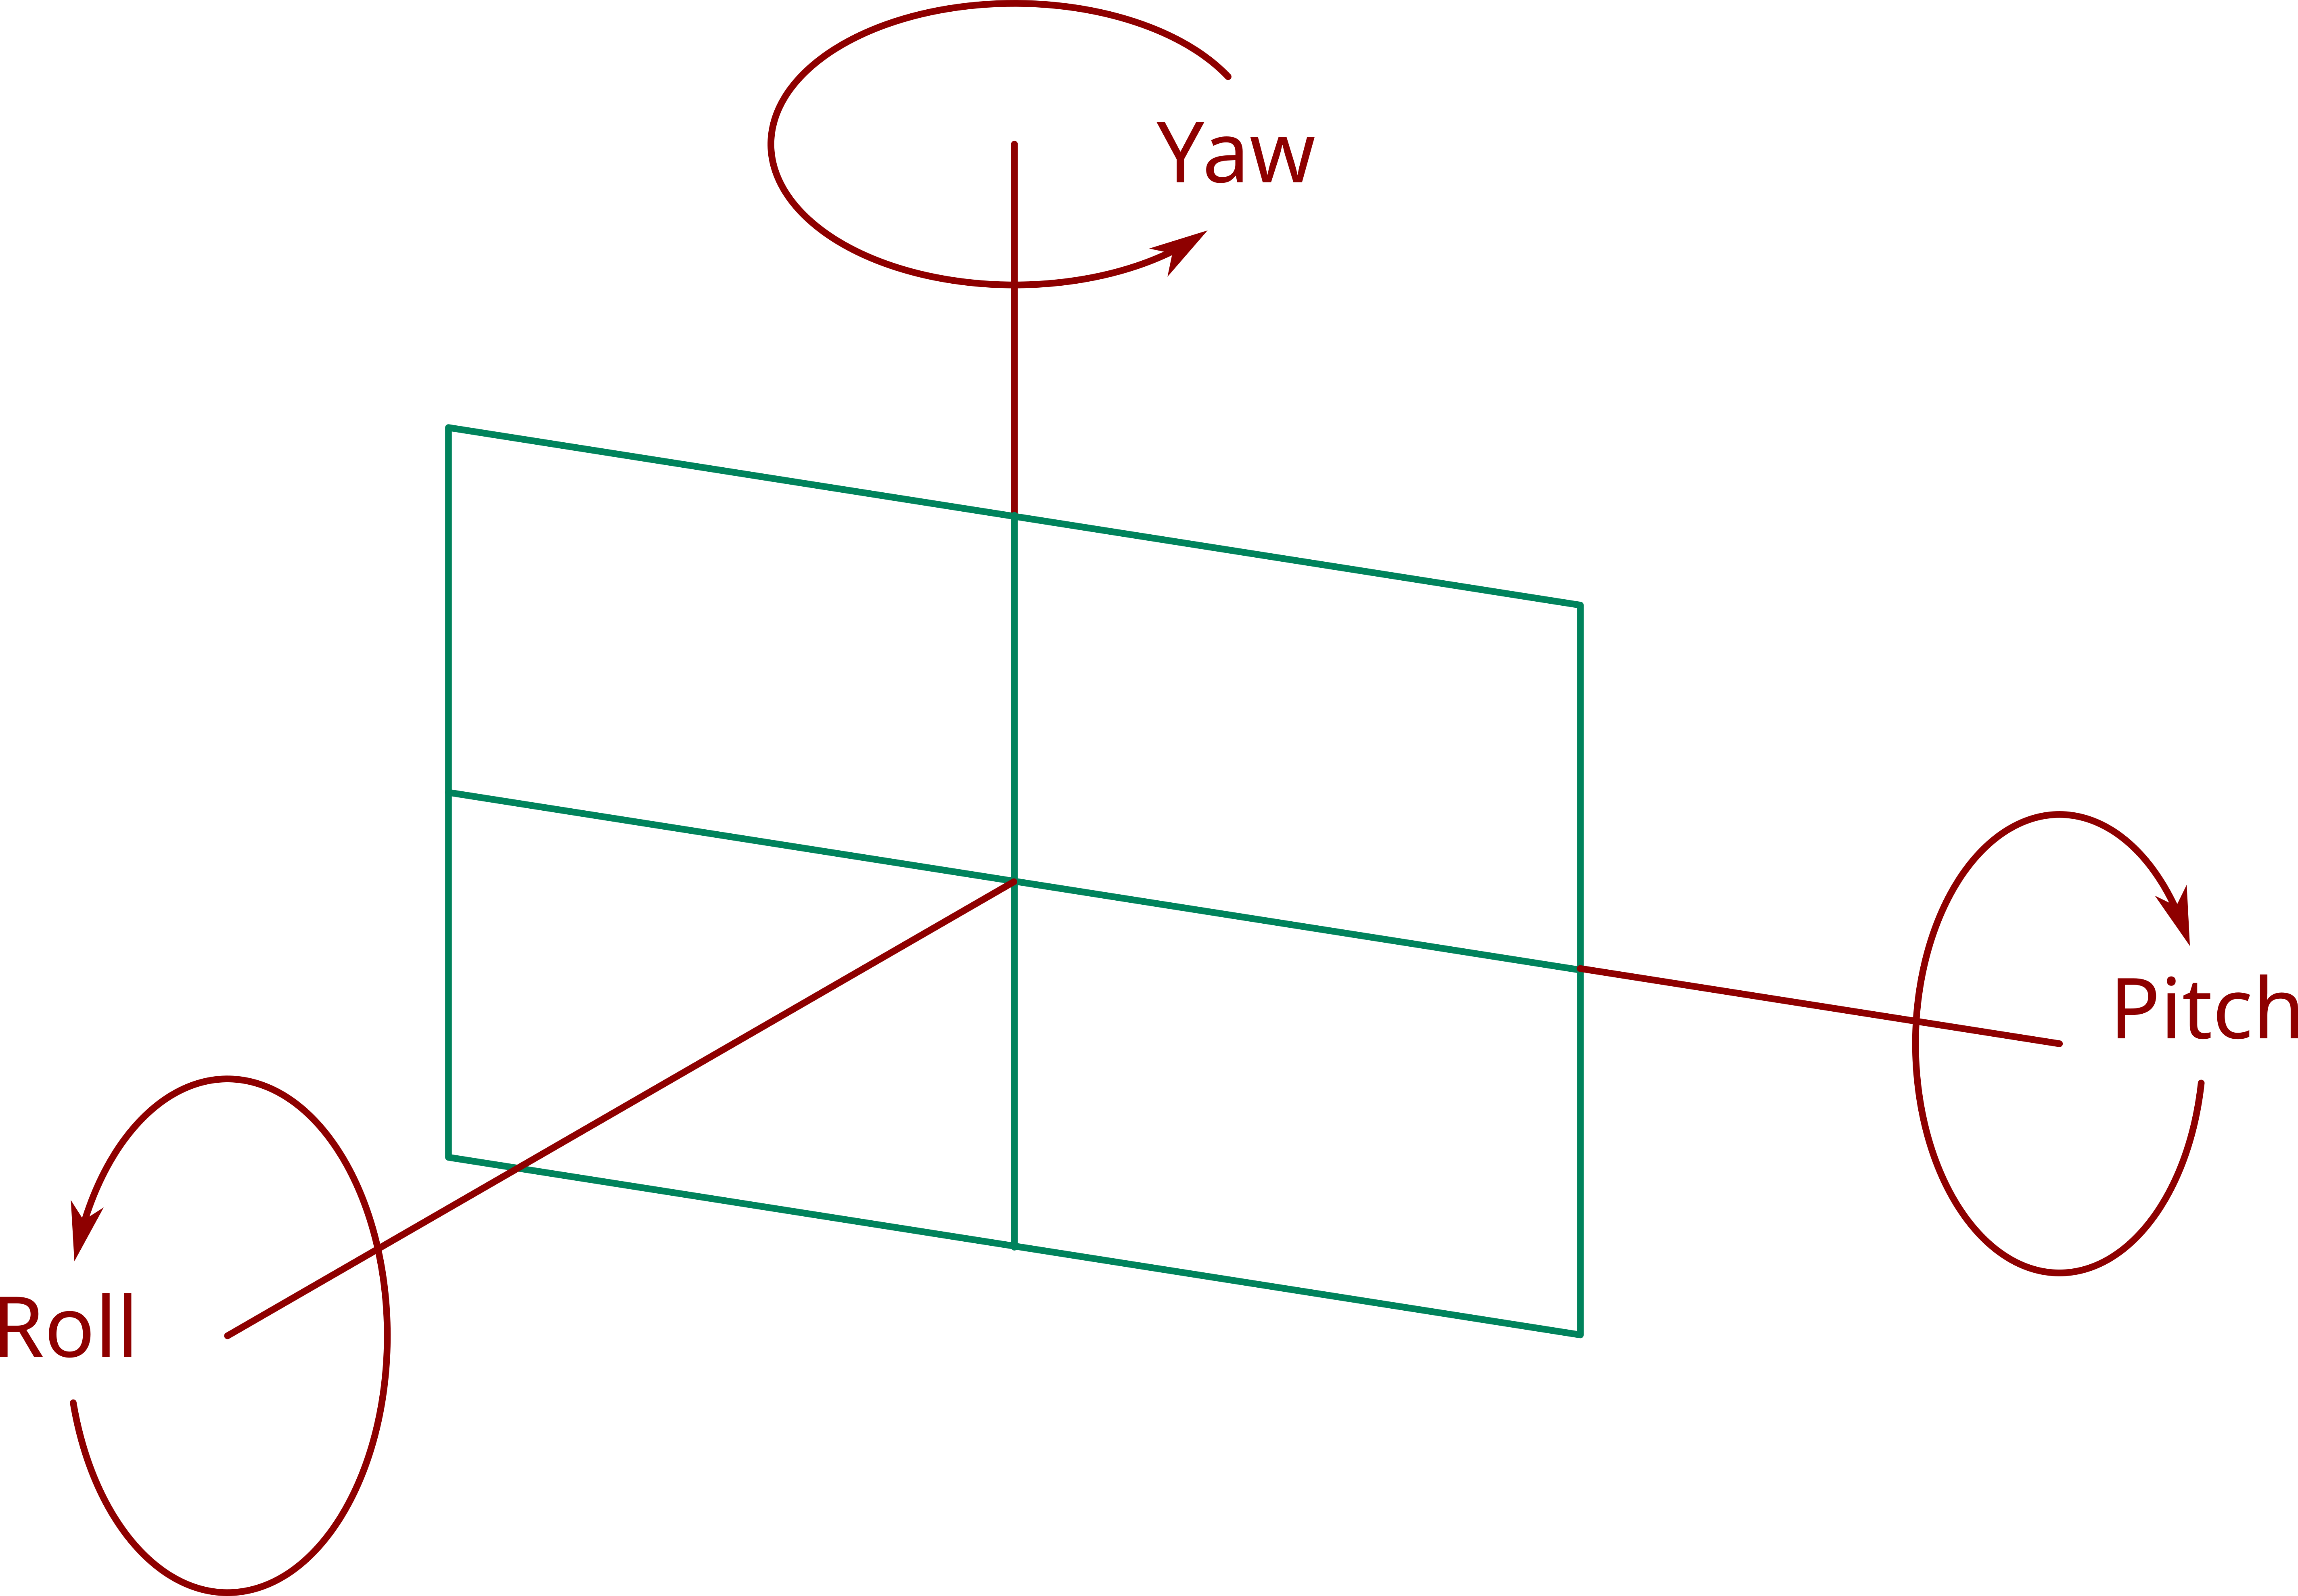
\includegraphics[width=.8\linewidth]{gfx/rollpitchyaw.png}
	\caption[Pitch, roll and yaw angles]{Pitch, roll and yaw angles}
	\label{fig:pitchrollyaw}
\end{figure}

This model let us compute the direction of the incoming rays just by indexing the particular pixel they hit, obtaining a map
\begin{equation}
	\label{eq:pixelmap}
	(p_x, p_y) \xmapsto{\mathfrak{h}_2} (\vartheta_{cs}, \varphi_{cs}),
\end{equation}
where $(p_x, p_y)$ are the components of the pixel in a system of coordinates whose origin is placed at the top-left corner of the sensor.

By composing \autoref{eq:initmap} and \autoref{eq:pixelmap}, we define the map
\begin{equation}
	(p_x, p_y) \xmapsto{\mathfrak{h} = \mathfrak{h_1}\circ\mathfrak{h_2}} (\vartheta', \varphi'),
\end{equation}
that summarises all the work the algorithm does: from a pixel on the camera's reference frame, we compute the origin of the incoming ray that hit that pixel.

\subsection{Pixel to Ray Map}
\label{subcsec:pixeltoray}

Let us consider a pixel $P$ whose coordinates on the sensor's reference frame are, in physical units, $(p_x, p_y)$, as depicted in \autoref{fig:pinhole}.

\begin{figure}[bth]
	\myfloatalign
	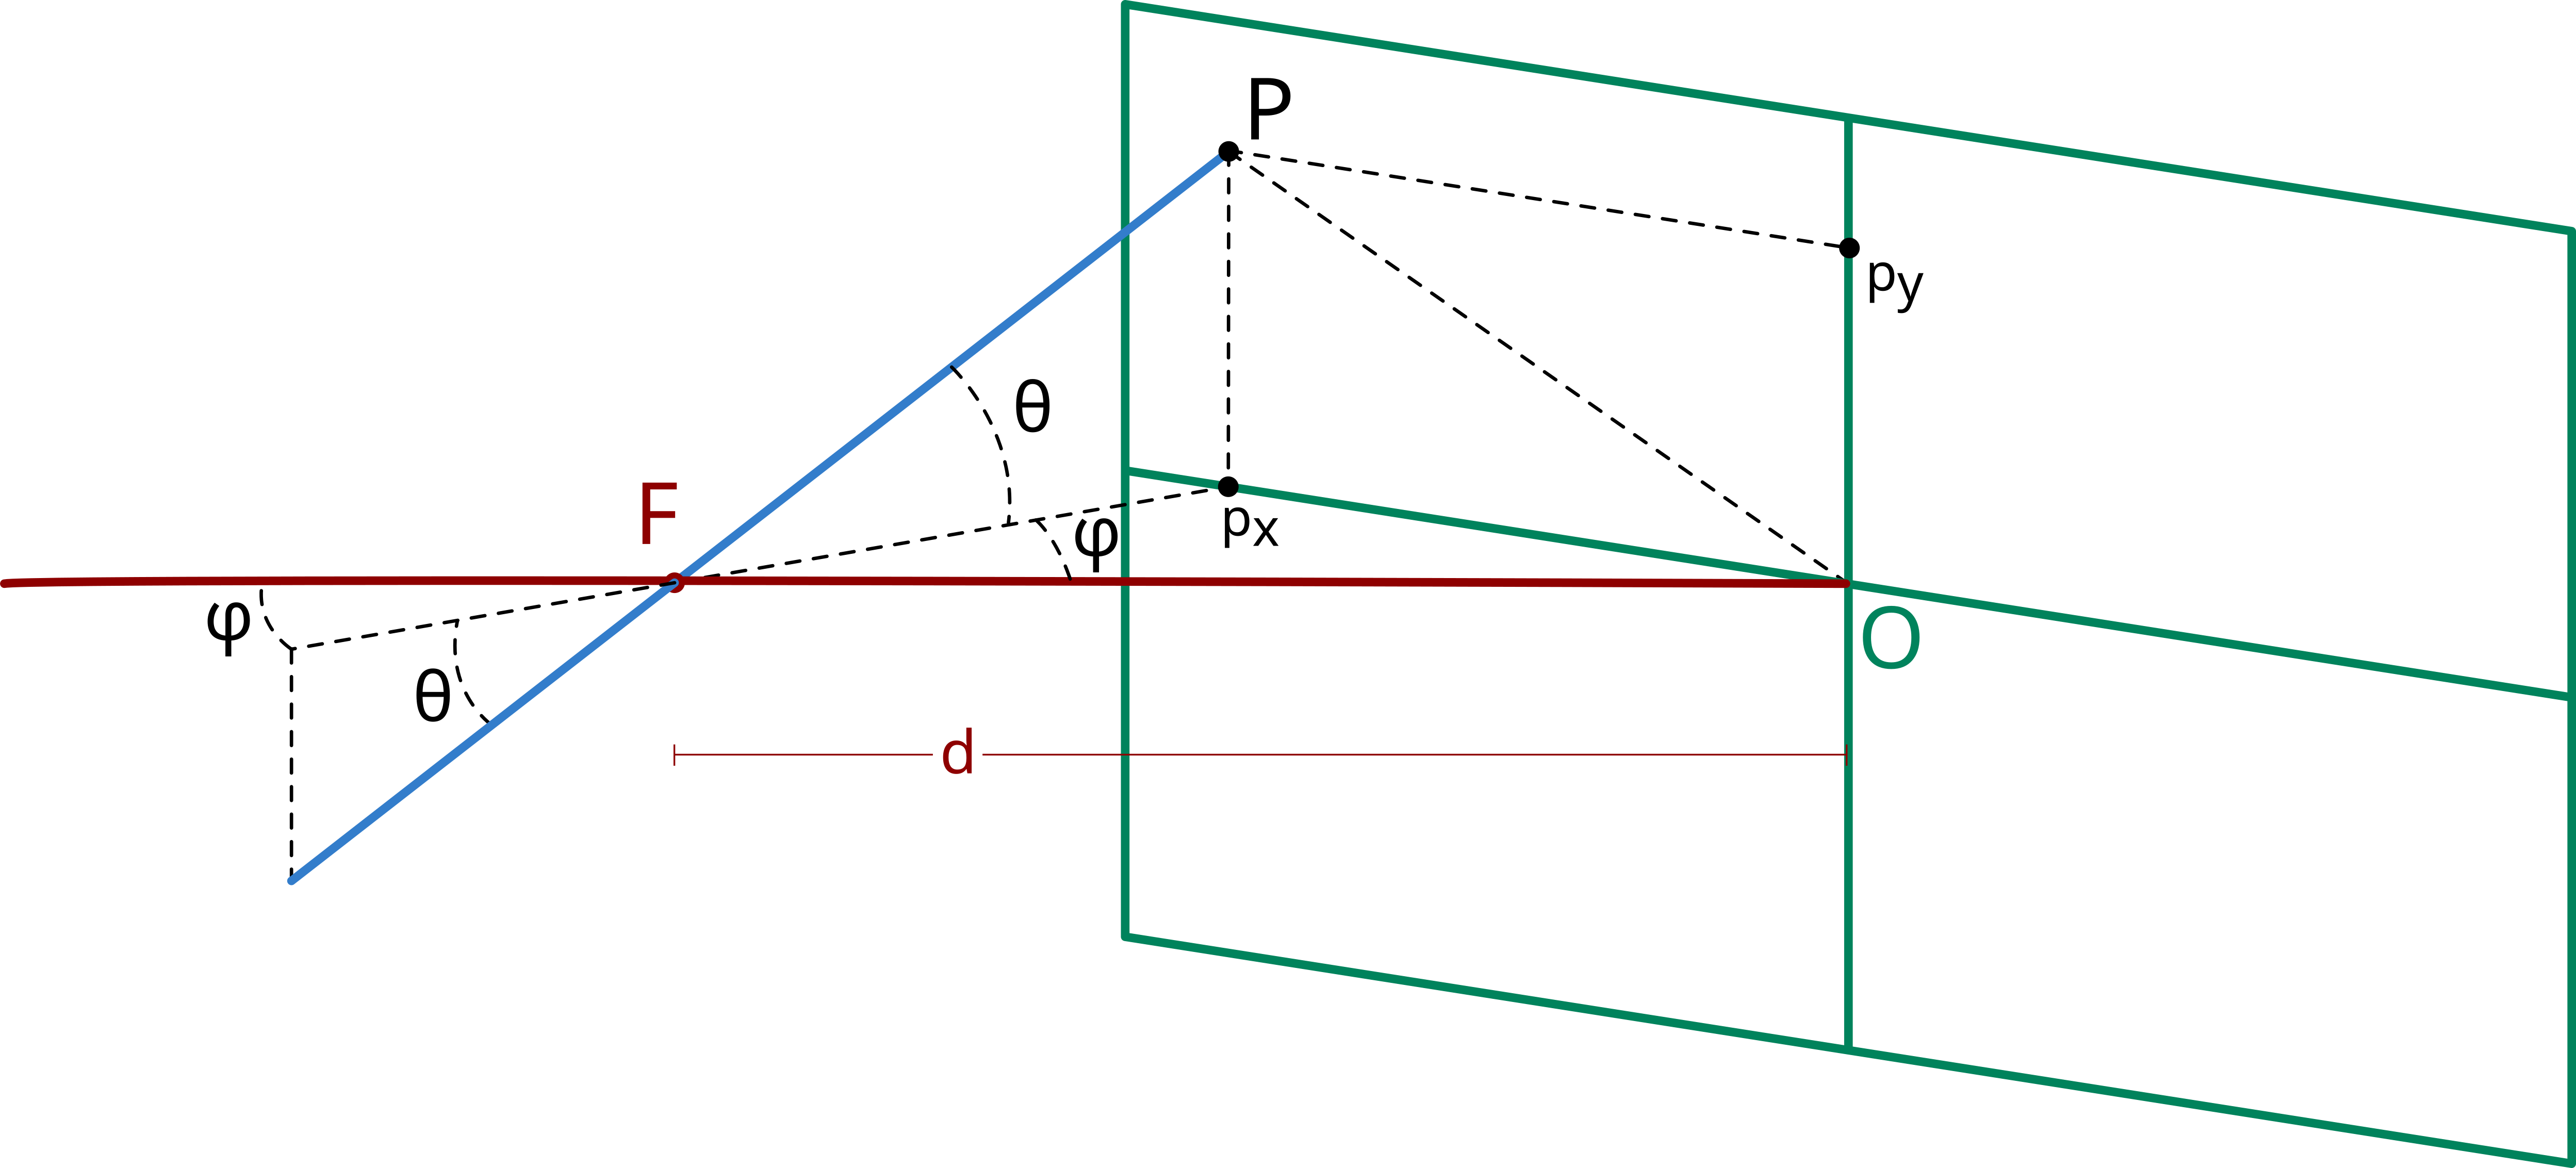
\includegraphics[width=.8\linewidth]{gfx/pinhole.png}
	\caption[Pinhole camera model]{Pinhole camera model}
	\label{fig:pinhole}
\end{figure}

All rays that hit the sensor are assumed, by our model, to pass through the focal point $F$. Thus, we can compute the angles $\vartheta$ and $\varphi$ for the ray hitting the sensor at pixel $P$ with elementary trigonometry.

From triangle $Fp_xO$ in \autoref{fig:pinhole}, we can obtain the angle $\varphi$ as
\[
	\varphi = \arctan{\frac{p_x}{d}}.
\]

Similary, the value of $\vartheta$ comes from the triangle $Fp_xP$ in \autoref{fig:pinhole}, which results in the following formula:
\[
	\vartheta = \arctan{\frac{p_y}{\sqrt{p_x^2 + d^2}}}.
\]

Finally, we need to adjust the zero for both $\vartheta$ and $\varphi$ to agree with the angle convention of the coordinate system. Therefore, the final formulas to computing the direction of an incoming ray hitting the camera's sensor ar a pixel $P = (p_x, p_y)$ are the following:
\begin{align}
	\vartheta_{cs} &= \frac{\pi}{2} + \arctan{\frac{p_y}{\sqrt{p_x^2 + d^2}}}, \\
	\varphi_{cs} &= \pi + \arctan{\frac{p_x}{d}}.
\end{align}

This discussion assumed the pixel coordinates to have its origin at the centre of the sensor. This is not the common coordinate system for pixels, as it usually have its origin at the top-left corner. A simple translation fixes that.

Furthermore, the pitch, roll and yaw angles were assumed to be zero. However, the addition of these angles is not difficult:
\begin{itemize}
	\item The roll angle, noted as $\alpha$, defines the rotation of the sensor on the image plane, so every pixel $(p_x, p_y)$ has to be rotated accordingly:
	\[
		\begin{pmatrix}
			p'_x \\
			p'_y
		\end{pmatrix} = 
		\begin{pmatrix}
			\cos\alpha & -\sin\alpha \\
			\sin\alpha & \cos\alpha 
		\end{pmatrix}
		\begin{pmatrix}
			p_x \\
			p_y
		\end{pmatrix}
	\]
	\item The pitch angle, noted as $\eta$, has to be simply added to the $\vartheta$ coordinate, as it defines the rotation of the sensor on that axis.
	\item The yaw angle, noted as $\lambda$, is the rotation of the sensor with respect to the $\varphi$ axis, so it has to be added to that coordinate.	
\end{itemize}

Taking all this into account, the final formulas to compute $(\vartheta_{cs}, \varphi_{cs})$ from the physical coordinates of the pixel $(p_x, p_y)$ are
\begin{align}
	\vartheta_{cs} &= \eta + \frac{\pi}{2} + \arctan{\frac{p_y}{\sqrt{p_x^2 + d^2}}}, \\
	\varphi_{cs} &= \lambda + \pi + \arctan{\frac{p_x}{d}}.,
\end{align}
where
\[
	p'_x = p_x\cos\alpha - p_y\sin\alpha, \qquad
	p'_y = p_x\sin\alpha + p_y\cos\alpha.
\]

\section{Initial Conditions Computation}
\label{sec:initcond}

The algorithm kernel integrates, backwards in time, an \ac{ODE} system. We already know the system we are working with, \autoref{theo:eqsmotion}, but for such a system to be uniquely solved, a set of initial conditions is needed.

That is, for each ray we need to know its components, \[(r, \vartheta, \varphi, p_r, p_\vartheta),\] at the time $\tau = 0$.

All rays hitting the camera share the same $r$, namely the position of the camera $r_c$.

In \autoref{subcsec:pixeltoray}, the initial $\vartheta_{cs}$ and $\varphi_{cs}$ for each ray were computed.

Therefore, we only need to compute the initial momentum components, $p_r$ and $p_\vartheta$, for each ray. In short, assuming we know the pixel the incoming ray is hitting and, thus, the $\vartheta_{cs}$ and $\varphi_{cs}$ components of the ray on the camera's local sky, we expect to obtain the map
\[
	(\vartheta_{cs}, \varphi_{cs}) \xmapsto{IC} (p_r, p_\vartheta).
\]

This is not a difficult task but a very delicate one, as some coordinate systems have to be taken into account and we should have a good understanding of them in order to properly compute the bases changes. A short summary of the work that follows is listed here:
\begin{enumerate}
	\item The initial position of the ray is known to be $(r_c, \vartheta_{cs}, \varphi_{cs})$. The components of the unit vector that points on the direction of motion of the camera, $B$, are noted as $(B_{\widehat{r}}, B_{\widehat{\vartheta}}, B_{\widehat{\varphi}})$, whereas its speed relative to the \ac{FIDO}, that is, the modulus of $B$, is noted as $\beta$.
	\item From $(\vartheta_{cs}, \varphi_{cs})$ we compute the unit vector in Cartesian coordinates, $N = (N^x, N^y, N^z)$, pointing to the direction of the incoming ray. This is computed on the camera's reference frame: a simple change to Cartesian coordinates is needed.
	\item The relativistic aberration caused by the motion of the camera and its speed around the black hole causes the \ac{FIDO} to measure the direction of motion of the incoming ray slightly different. The Cartesian components of this derived unit vector, $n = (n^x, n^y, n^z)$ need to be computed.
	\item Then, $n_F$ needs to be seen from the \ac{FIDO}'s orthonormal basis by means of the ligatures provided by the vector $B$ and the orthogonal relations. This gives us the components $(n^r, n^\vartheta, n^\varphi)$.
	\item From $n_F$ expressed on the right coordinate system, we need to compute the covariant components of the four momentum $(p_t, p_r, p_\vartheta, p_\varphi)$.
\end{enumerate}

Before going ahead with the details of the five steps above, let us set up the bases on the vector spaces we are working on. First of all, for the spacetime written in \ac{BL} coordinates, $(t, r, \vartheta, \varphi)$, we have the usual basis for the tangent space $T_p M$,
\begin{equation}
	\mathcal{B}_u = (\partial_t, \partial_r, \partial_\vartheta, \partial_\varphi).
\end{equation}

Furthermore, ee would like to work with an orthonormal spherical basis, that will be noted as
\begin{equation}
	\mathcal{B}_s = (e_t, e_r, e_\vartheta, e_\varphi).
\end{equation}

Finally, a Cartesian coordinate system placed on the camera's reference frame is needed. Its notation and components are:
\[
	\mathcal{B}_c = (e_t, e_x, e_y, e_z).
\]

Let us now compute the expressions of the vectors in $\mathcal{B}_s$ in terms of the basis $\mathcal{B}_u$. We want an orthonormal basis, so for the spatial coordinates, it is only necessary to divide by its module. Therefore, their expressions in terms of $\mathcal{B}_u$ are:
\begin{equation}
	e_r = \frac{\sqrt{\Delta}}{\rho} \partial_r, \quad
	e_\vartheta = \frac{1}{\rho} \partial_\vartheta, \quad
	e_\varphi = \frac{1}{\varpi} \partial_\varphi.
\end{equation}

For the time coordinate $e_t$ to be unitary and orthogonal to the spatial coordinates, we can define it as
\[
	e_t = a\partial_t + b\partial_\varphi,
\]
where $a$ and $b$ are unknowns.

Imposing the orthonormality property ($e_t$ has to be negative unitary to preserve the signature and, in particular, $e_t$ is perpendicular to $e_\varphi$), we can set up a system of equations to solve $a$ and $b$:
\begin{align}
	\label{eq:systemab}
	g(e_t, e_t) &= -1 \\ \nonumber
	g(e_t, e_\varphi) &= 0
\end{align}

From \autoref{eq:systemab}, we conclude that $a = \frac{1}{\alpha}$ and $b = \frac{\omega}{\alpha}$. Therefore, the orthonormal basis $\mathcal{B}_s$ vectors are:
\begin{equation}
	e_t = \frac{1}{\alpha}\partial_t + \frac{\omega}{\alpha}\partial_\varphi, \quad
	e_r = \frac{\sqrt{\Delta}}{\rho} \partial_r, \quad
	e_\vartheta = \frac{1}{\rho} \partial_\vartheta, \quad
	e_\varphi = \frac{1}{\varpi} \partial_\varphi.
\end{equation}

The change of basis matrix, that maps $\mathcal{B}_s$ coordinates to $\mathcal{B}_u$ components is then
\begin{equation}
	\mathcal{M} = \begin{pmatrix}
	\frac{1}{\alpha} & 0 & 0 & 0 \\
	0 & \frac{\sqrt{\Delta}}{\rho} & 0 & 0 \\
	0 & 0 & \frac{1}{\rho} & 0 \\
	\frac{\omega}{\alpha} & 0 & 0 & \frac{1}{\varpi}
	\end{pmatrix}.
\end{equation}

This operation can be seen as an endomorphism on the tangent space, where we map vectors expressed in the orthonormal basis to vectors in the \ac{BL} coordinates. If we denote by $N$ the tangent space with the basis $\mathcal{B}_s$ and by $E$ the tangent space with the basis $\mathcal{B}_u$\footnote{Note that $N$ and $E$ are the same vector space, but their notations are different to express the different bases chosen.}, then $\mathcal{M}$ is the matrix of the endomorphism \[T \colon N \to E.\]

\subsection{Incoming Ray Direction}

We can now begin with the first task: from the spherical coordinates of the ray on the camera's local sky, $(\vartheta_{cs}, \varphi_{cs})$, we can compute the Cartesian components of the unit vector $N = (N^x, N^y, N^z)$ that points in the direction of the incoming ray in the usual way:
\begin{equation}
	N^x = \sin\vartheta_{cs} \cos\varphi_{cs}, \quad N^y = \cos\vartheta_{cs} \sin\varphi_{cs}, \quad N^z = \cos\vartheta_{cs}.
\end{equation}

\subsection{Relativistic Aberration}

We have two observers: one local to the camera, that is measuring the ray's direction of motion as the vector $N$ and the \ac{FIDO}, which will see it as the vector $n = (n^x, n^y, n^z)$. As the camera moves at speed $\beta$, on the direction of $e_y$, with respect to the \ac{FIDO}, the Lorentz transformation can be written as
\begin{align}
	\label{eq:lorentz}
	dt' &= \frac{dt - \beta dy}{\upsilon}, \\ \nonumber
	dx' &= dx, \\ \nonumber
	dy' &= \frac{dy - \beta dt}{\upsilon}, \\ \nonumber
	dz' &= d';
\end{align}
where $\upsilon = \sqrt{1 - \beta^2}$, $(dt', dx', dy', dz')$ are the \ac{FIDO} coordinates and $(dt, dx, dy, dz)$ are the coordinates local to the camera.

We can finally obtain the components $(n^x, n^y, n^z)$ just by applying \autoref{eq:lorentz}:
\begin{align*}
	n^x &= \frac{dx'}{dt'} = \frac{\sigma dx}{dt - \beta dy} = \frac{\frac{dx}{dt} \upsilon}{1 - \beta \frac{dy}{dt}} = \frac{N^x \upsilon}{1 - \beta N^y}, \\
	n^y &= \frac{dy'}{dt'} = \frac{dy - \beta dt}{dy}{dt - \beta dy} = \frac{N^y - \beta}{1 - \beta N^y}, \\
	n^z &= \frac{dz'}{dt'} = \frac{\sigma dz}{dt - \beta dy} = \frac{\frac{dz}{dt} \upsilon}{1 - \beta \frac{dy}{dt}} = \frac{N^z \upsilon}{1 - \beta N^y}.
\end{align*}

The vector $N$ points in the direction of the incoming ray; particularly, it is pointing to the origin of the ray. The ray does not move \emph{to} its origin but \emph{from} there, so in order to have $n_F$ to point in the direction of motion of the ray, we must multiply $n$ by $-1$. This gives us the final equations for the relativistic aberration \cite[Eq. (A.9)]{thorne15}:
\begin{align}
	n^x &= \frac{-\sqrt{1 - \beta^2}N^x}{1 - \beta N^y}, \\
	n^y &= \frac{- N^y + \beta}{1 - \beta N^y}, \\
	n^z &= \frac{-\sqrt{1 - \beta^2} N^z}{1 - \beta N^y}. \\
\end{align}

\subsection{Change of Basis}

We have now the direction of the ray as seen by the \ac{FIDO} in the basis $\mathcal{B}_c$, but we want to express it in the spherical orthonormal coordinate system, whose basis is $\mathcal{B}_s$.

We need then to express one basis in terms of the other, using the orthonormality constraints and the direction of motion of the camera, $B$, whose coordinates are noted as $(B^r, B^\theta, B^\varphi)$.

First of all, we define $e_y$ to be $B$, so it is directly written in terms of the basis $\mathcal{B}_s$:
\begin{equation}
	\label{eq:changey}
	e_y = B^r e_r + B^\vartheta e_\vartheta + B^\varphi e_\varphi.
\end{equation}

We define $e_x$ to be perpendicular to $e_y$ and in the plane spanned by $e_r$ and $e_\varphi$, so we can write
\begin{equation*}
	e_x = e_x^r e_r + e_x^\varphi e_\varphi,
\end{equation*}
where $e_x^r$ and $e_x^\varphi$ are the unknown coordinates. Using the orthonormality constraints, that is,
\begin{align*}
	0 &= e_y e_x = B^r e_x^r + B^\varphi e_x^\varphi, \\
	1 &= e_x e_x = \left( e_x^r \right)^2 + \left(e_x^\varphi\right)^2;
\end{align*}
we conclude that $e_x^r = \frac{B^\varphi}{\upsilon}$ and  $e_x^\varphi = -\frac{B^r}{\upsilon}$, so the $e_x$ component is written as
\begin{equation}
	\label{eq:changex}
	e_x = \frac{B^\varphi}{\upsilon} e_r - \frac{B^r}{\upsilon} e_\varphi.
\end{equation}

We proceed similarly to compute the spherical coordinates of $e_z$. Using the orhonormalization constraints, we have the system
\begin{align*}
	0 &= e_y e_z = B^r e_z^r + B^\vartheta e_z^\vartheta + B^\varphi e_z^\varphi, \\
	0 &= e_x e_z = \frac{B^\varphi}{\upsilon} e_z^r - \frac{B^r}{\upsilon} e_z^\varphi, \\
	1 &= e_z e_z = \left(e_z^r\right)^2 + \left(e_z^\vartheta\right)^2 + \left(e_z^\varphi\right)^2,
\end{align*}
whose solution gives us the components of $e_z$:
\begin{equation}
	\label{eq:changez}
	e_z = \frac{B^r B^\vartheta}{\upsilon} e_r - \upsilon e_\vartheta + \frac{B^\vartheta B^\varphi}{\upsilon} e_\varphi.
\end{equation}

Using equations \ref{eq:changey}, \ref{eq:changex} and \ref{eq:changez}, it is then trivial to compute the components of $n$ in the spherical orthonormal basis $\mathcal{B}_s$:
\begin{align}
	n^r &= \frac{B^\varphi}{\upsilon} n^x + B^r n^y + \frac{B^r B^\vartheta}{\upsilon} n^z, \\
	n^\vartheta &= B^\vartheta n^y - \upsilon n^z, \\
	n^\varphi &= \frac{B^r}{\upsilon} n^x + B^\varphi n^y + \frac{B^\vartheta B^\varphi}{\upsilon} n^z.
\end{align}

\subsection{Momentum}

We finally have the direction of motion of the ray expressed in the proper basis, but in order to compute the initial conditions, we need its four momentum; that is, we want to obtain the function $f$ that maps $N$ to the dual space of $E$: $E^*$, as seen in \autoref{fig:diagram}, where $T$ is the endomorphism defined before and $\phi_N$, $\phi_E$ are the isomorphisms between the base spaces and their dual versions.

\begin{figure}[bth]
	\myfloatalign
	\begin{tikzpicture}
	\matrix (m) [matrix of math nodes,row sep=3em,column sep=4em,minimum width=2em]
	{
		N & E \\
		N^* & E^* \\};
	\path[-stealth]
	(m-1-1) edge node [left] {$\phi_N$} (m-2-1)
	edge [double] node [above] {$T$} (m-1-2)
	(m-2-2.west|-m-2-2) edge node [below] {$T^*$}
	(m-2-1)
	(m-1-2) edge node [right] {$\phi_E$} (m-2-2)
	(m-1-1) edge [right,dashed,->] node {$f$} (m-2-2);
	\end{tikzpicture}
	\caption[Conmutative diagram]{Conmutative diagram}
	\label{fig:diagram}
\end{figure}

Remember that $N$ has the orthonormal basis, so the expression of $\phi_N$ is trivial: only the sign of the time coordinate has to be changed. The expression of $\phi_E$ is more difficult, and that is why we are going to compute $f$ as
\begin{equation}
	f = (T^*)^{-1} \circ \phi_N.
\end{equation}

Using matrix notation, we have
\begin{equation}
	\mathcal{M}_f = \left(\mathcal{M}^t\right)^{-1} \mathcal{M}_{\phi_N},
\end{equation}
where
\[
	\left(\mathcal{M}^t\right)^{-1} = \begin{pmatrix}
		\alpha & 0 & 0 & -\omega\varpi \\
		0 & \frac{\rho}{\sqrt{\Delta}} & 0 & 0 \\
		0 & 0 & \rho & 0 \\
		0 & 0 & 0 & \varpi
	\end{pmatrix}
\]
and
\[
	\mathcal{M}_{\phi_N} = \begin{pmatrix}
	-1 & 0 & 0 & 0\\
	0 & 1 & 0 & 0\\
	0 & 0 & 1 & 0\\
	0 & 0 & 0 & 1
	\end{pmatrix}.
\]

The moment of the ray is then $f(n)$, that is,
\begin{equation}
	\begin{pmatrix}
		p_t \\
		p_r \\
		p_\vartheta \\
		p_\varphi \\
	\end{pmatrix} = \begin{pmatrix}
		-\alpha & 0 & 0 & -\omega\varpi \\
		0 & \frac{\rho}{\sqrt{\Delta}} & 0 & 0 \\
		0 & 0 & \rho & 0 \\
		0 & 0 & 0 & \varpi
	\end{pmatrix}
	\begin{pmatrix}
		1 \\
		n^r \\
		n^\vartheta \\
		n^\varphi
	\end{pmatrix} = \begin{pmatrix}
		-\alpha - \omega\varpi n^\varphi \\
		\frac{\rho}{\sqrt{\Delta}} n^r \\
		\rho n^t \\
		\varpi n^\varphi
	\end{pmatrix}
\end{equation}

We know that Kerr is stationary, so $p_t$ is conserved (see \autoref{eq:conservedpt}). We will normalize it by defining
\[
	E_f = - \frac{1}{p_t}
\]  
as the energy measured by the \ac{FIDO} and multiplying $p$ by $E_f$. The final components of the momentum \cite[Eq. (A.11)]{thorne15} are:
\begin{align}
	p_t &= -1, \\
	p_r &= E_f \frac{\rho}{\sqrt{\Delta}} n^r, \\
	p_\vartheta &= E_f \rho n^t, \\
	p_\varphi &= E_f \varpi n^\varphi.
\end{align}

Because of the axial symmetry on Kerr black holes (see \autoref{eq:conservedpphi}), $p_\varphi$ is another conserved quantity. With this and the Carter's constant, defined at \autoref{eq:carter}, and using that the mass of the lightlike particles is zero and the energy is unitary, we can define the two ray's conserved quantities \cite[Eq. (A.12)]{thorne15}:
\begin{equation}
	b \defeq p_\varphi, \quad q \defeq p_\vartheta^2 + \cos^2\vartheta \left( \frac{b^2}{\sin^2\vartheta} - a^2 \right).
\end{equation}

\section{Numerical Solver}
\label{sec:numerical}

Once we have the \ac{ODE} system and the initial conditions for the ray we want to solve, the final step is to numerically integrate, backwards in time, the geodesic followed by the ray.

The problem reduces then to numerically integrate an \ac{ODE} system, which is a well-known problem and widely studied in the literature.

In order to accomplish this task, the algorithm used by our ray tracer uses a classic Runge-Kutta method, along with an automated step size computation based on the estimated error of the step.

The Runge-Kutta method is based on the \texttt{DOPRI5} algorithm, described in \cite{hairer93} and \cite{hairer96}.

The automated control for the step size based on the estimated error follows the ideas in \cite[Sec. II.4, Subsec. Automatic Step Size Control]{hairer93}.

Furthermore, the step size is stabilized using the algorithm described in \cite[Sec. IV.2]{hairer96}.

\subsection{Adaptive Runge-Kutta Method}

The Runge-Kutta methods solve general \ac{IVP} like the following one,
\begin{align*}
	\dot{y} = f(t,y) \\
	y(t_0) = y_0,
\end{align*}
where $y$ can be scalar or vector and $f$, $t_0$ and $y_0$ are known.

Given a pair $(t_n, y_n)$, the adaptive Runge-Kutta methods compute the value of the system at time $t_{n+1}$ as follows:
\begin{align*}
	y_{n+1} = y_n + h \sum_{i=1}^s b_i k_i\\
	y^*_{n+1} = y_n + h \sum_{i=1}^s b^*_i k_i,
\end{align*}

where $y_{n+1}$ is the new estimated value and $y^*_{n+1}$ is a higher order approximation that is used to estimate the error of the result, which is computed as $\vert y^*_{n+1} - y_{n+1} \vert$. In this notation, $h$ is the so-called \emph{step}, which is the amount of time the system is advanced, and the components $k_i$ are defined as follows:
\[
	k_i = f(t_n + c_ih, y_n + h\sum_{j=1}^{i-1} a_{ij} k_j).
\]

The coefficients $a_{ij}$, $b_i$, $b_i^*$ and $c_i$ define the model, and are usually arranged on what is called a Butcher's table (see \autoref{tab:generalbutcher} for a generic example).

\begin{table}[bth]
	\myfloatalign
	\begin{tabularx}{.54\textwidth}{c|ccccc}
		$0$&  & & & & \\
		$c_2$& $a_{21}$ & & & & \\
		$c_3$& $a_{31}$ & $a_{32}$ & & & \\
		$\vdots$& $\vdots$ &  & $\ddots$ & & \\
		$c_s$& $a_{s1}$  & $a_{s2}$ & $\cdots$ & $a_{s(s-1)}$ & \\ \hline
		& $b_1$ & $b_2$ & $\cdots$ & $b_{s-1}$ & $b_s$ \\ \hline
		& $b^*_1$ & $b^*_2$ & $\cdots$ & $b^*_{s-1}$ & $b^*_s$ \\
	\end{tabularx}
	\caption{Butcher's table for a generic adaptive Runge-Kutta method}
	\label{tab:generalbutcher}
\end{table}

Our system of \ac{ODE}, \autoref{theo:eqsmotion}, follows this model:
\begin{enumerate}
	\item $\dot{y} = (\dot{r}, \dot{\vartheta}, \dot{\varphi}, \dot{p}_r, \dot{p}_\vartheta)$,
	\item $f(t,y)$ is the right hand side of the equations and actually it does not depend on $t$, thus it can be written as $f(y)$.
	\item $t_0 = 0$ and $y_0 = (r_c, \vartheta_{cs}, \varphi_{cs}, p_{r}, p_{\vartheta})$ are the initial conditions computed in \autoref{sec:initcond}.
\end{enumerate}

The selected Runge-Kutta algorithm is a fourth order method with an estimation of the error based on a fifth order approximation, and whose Butcher's table is described on \autoref{tab:butcher}.

\begin{table}[bth]
	\myfloatalign
	\begin{tabularx}{.9\textwidth}{c|ccccccc}
		$0$&  & & & & & & \\
		$\frac{1}{5}$&  $\frac{1}{5}$& & & & & & \\
		$\frac{3}{10}$&  $\frac{3}{40}$&  $\frac{9}{40}$& & & & & \\
		$\frac{4}{5}$&  $\frac{44}{45}$&  $-\frac{56}{15}$&  $\frac{32}{9}$& & & & \\
		$\frac{8}{9}$&  $\frac{19372}{6561}$&  $-\frac{25360}{2187}$&  $\frac{64448}{6561}$&  $-\frac{212}{729}$& & & \\
		$1$&  $\frac{9017}{3168}$&  $-\frac{355}{33}$&  $\frac{46732}{5247}$&  $\frac{49}{176}$&  $-\frac{5103}{18656}$& & \\
		$1$&  $\frac{35}{384}$&  $0$&  $\frac{500}{1113}$&  $\frac{125}{192}$&  $-\frac{2187}{6784}$&  $\frac{11}{84}$& \\ \hline
		$y_1$&  $\frac{35}{384}$&  $0$&  $\frac{500}{1113}$&  $\frac{125}{192}$&  $-\frac{2187}{6784}$&  $\frac{11}{84}$&  $0$ \\ \hline
		$\widehat{y}_1$&  $\frac{5179}{57600}$&  $0$&  $\frac{7571}{16695}$&  $\frac{393}{640}$&  $-\frac{92097}{339200}$&  $\frac{187}{2100}$&  $\frac{1}{40}$
	\end{tabularx}
	\caption{Butcher's table for the ray tracer solver}
	\label{tab:butcher}
\end{table}

\subsection{Stabilization algorithm}